\documentclass[conference]{IEEEtran}
\IEEEoverridecommandlockouts
\usepackage{cite}
\usepackage{amsmath,amssymb,amsfonts}
\usepackage{algorithmic}
\usepackage{graphicx}
\usepackage{textcomp}
\usepackage{xcolor}

\def\BibTeX{{\rm B\kern-.05em{\sc i\kern-.025em b}\kern-.08em
    T\kern-.1667em\lower.7ex\hbox{E}\kern-.125emX}}

\begin{document}

\title{CareLog A Multi Role Care Coordination Platform for Home Based Elderly Monitoring}

\author{
\IEEEauthorblockN{Tella Sindhu Priya}
\IEEEauthorblockA{\textit{Department of Computer Science and Engineering} \\
\textit{B V Raju Institute of Technology} \\
Narsapur, Medak, Telangana, India \\
24211A05KA@bvrit.ac.in}
\and
\IEEEauthorblockN{Thallapelli Akash}
\IEEEauthorblockA{\textit{Department of Computer Science and Engineering} \\
\textit{B V Raju Institute of Technology} \\
Narsapur, Medak, Telangana, India \\
24211A05KC@bvrit.ac.in}
\and
\IEEEauthorblockN{Ramya Sree}
\IEEEauthorblockA{\textit{Department of Computer Science and Engineering} \\
\textit{B V Raju Institute of Technology} \\
Narsapur, Medak, Telangana, India \\
24211A05JP@bvrit.ac.in}
\and
\IEEEauthorblockN{S Arun Kumar}
\IEEEauthorblockA{\textit{Department of Computer Science and Engineering} \\
\textit{B V Raju Institute of Technology} \\
Narsapur, Medak, Telangana, India \\
24211A05JH@bvrit.ac.in}
}

\maketitle

\begin{abstract}
CareLog is a software only platform that improves coordination in home based elderly care. Care is often delivered by multiple caregivers and critical details are lost during shift changes. Family members and doctors also lack timely visibility into daily care. CareLog addresses these gaps through structured daily checklists, voice based observations, vitals logging with safety validation, real time alerts, and weekly summary reports. The system supports three main roles: caregiver, family member, and doctor. Caregivers record tasks and vitals using a simple checklist and optional voice input. Abnormal vitals trigger alerts to family and doctor. Doctors review logs, validate entries, and add clinical notes. All data is stored in a cloud database and summarized in a weekly report for review. This paper presents the architecture, module design, and workflow of CareLog, and explains how it reduces information loss without relying on hardware devices.
\end{abstract}

\begin{IEEEkeywords}
care coordination, elderly monitoring, voice documentation, real time alerts, weekly care report
\end{IEEEkeywords}

\section{Introduction}
Caring for elderly patients at home is demanding and often involves multiple caregivers working in shifts. In many homes, shift handoff is verbal and incomplete. Important details such as medication timing, meal completion, or symptoms are not passed clearly to the next caregiver. Families are usually not present and depend on short phone calls for updates. Doctors often receive updates only during visits, with no structured daily record. CareLog is designed to solve this coordination gap with a software only system that keeps care structured, visible, and timely.

\section{Literature Review}
Recent work in remote patient monitoring highlights the importance of structured data capture and timely alerts \cite{b1,b3}. Studies on voice based documentation show reduced workload when speech is confirmed before storage \cite{b4}. Automated summaries improve clinical review when daily data is structured \cite{b2}. However, most solutions focus on wearable devices or clinical settings rather than home care workflows. This gap motivates a system that combines daily care logging, alerts, and weekly summaries without new hardware.

\section{Existing Work}
Manual logs and verbal handoffs are still common because they are simple, but they are inconsistent and hard to track. Messaging apps provide updates but lack structure. Wearable based monitoring systems offer continuous vitals but require devices, charging, and compliance. Hospital portals focus on clinical records, not daily home care. There is no widely used system that connects caregivers, family members, and doctors in one unified workflow with structured daily logs and weekly reports.

\section{Problem Statement}
Home based elderly care is fragmented because caregivers work in shifts and updates are shared verbally or through scattered notes. Important information about medication, meals, symptoms, or vitals is often lost. Family members and doctors do not have a real time view of daily care, which delays decisions and reduces trust. Existing solutions either depend on expensive hardware or provide unstructured communication that cannot be summarized effectively. The problem is to design a software only system that captures daily care in a structured form, validates vitals, generates real time alerts, and produces a clear weekly summary for families and doctors. The system must remain easy for caregivers and preserve privacy through role based access.

\section{Methodology}

\subsection{System Overview}
CareLog is a multi role care coordination platform built for three primary roles: caregiver, family member, and doctor. Each role has a tailored dashboard. The system captures daily tasks, vitals, and observations, and provides alerts and weekly summaries.

\subsection{Architecture}
The platform uses cloud authentication, a real time database, and messaging services. Client applications connect to the backend for storage and updates. A reporting service generates weekly summaries in a report file. The Level 0 data flow diagram in Fig.~\ref{fig:dfd0} follows standard DFD rules with external entities, a single process, and a data store.

\begin{figure}[htbp]
\centerline{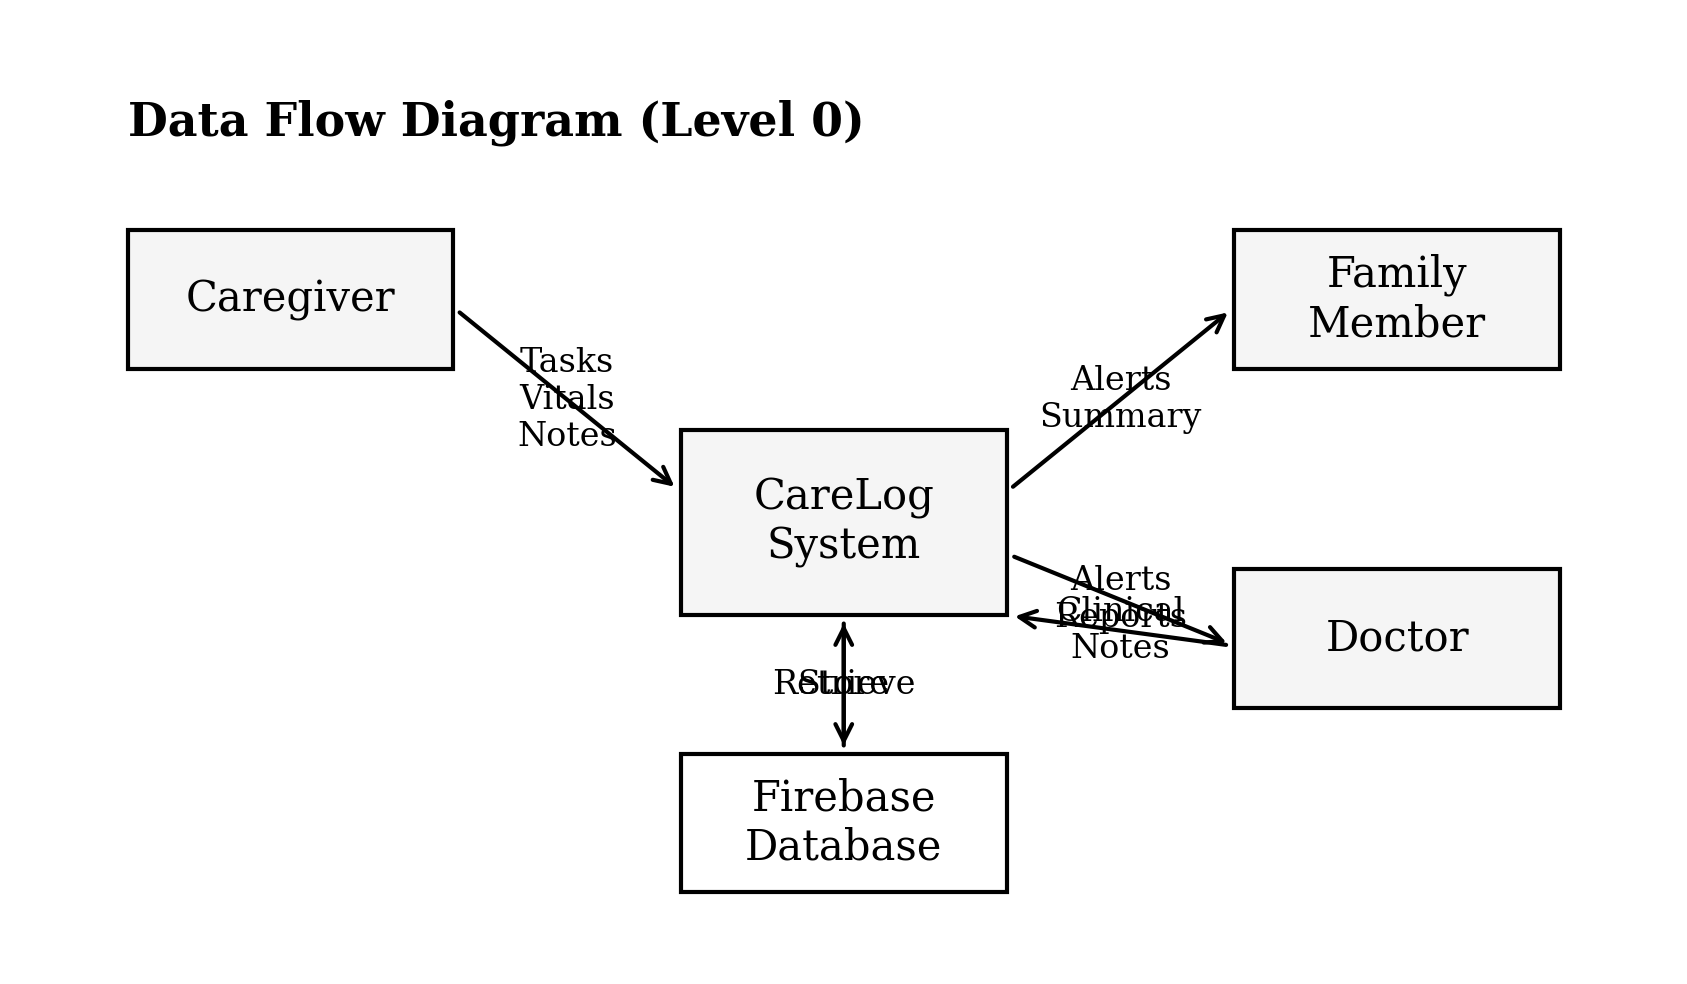
\includegraphics[width=\columnwidth]{output/figures/fig1_dfd_level0.png}}
\caption{Data Flow Diagram (Level 0) for CareLog.}
\label{fig:dfd0}
\end{figure}

\subsection{Use Case Model}
The UML use case diagram in Fig.~\ref{fig:usecase} shows the roles and their core interactions with the system. Caregivers log tasks, enter vitals, and record handoff notes. Family members view alerts and weekly reports. Doctors review alerts and add clinical notes.

\begin{figure}[htbp]
\centerline{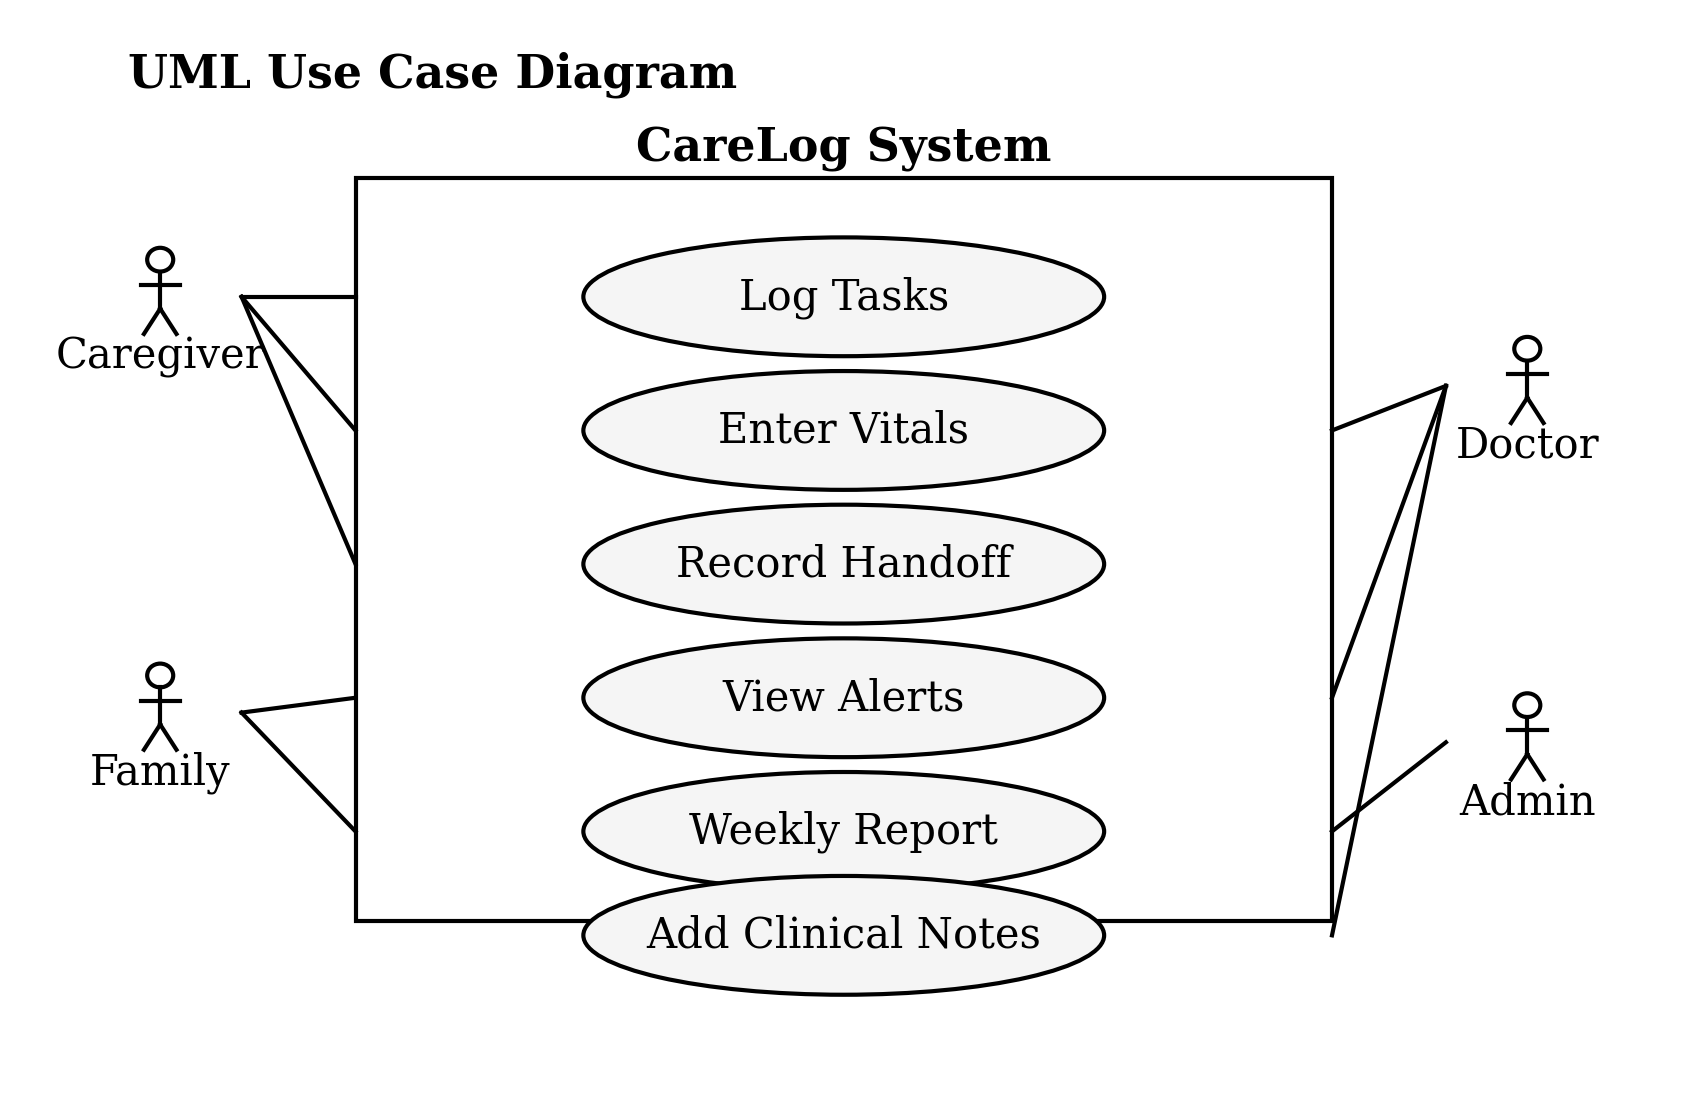
\includegraphics[width=\columnwidth]{output/figures/fig2_uml_use_case.png}}
\caption{UML Use Case Diagram of CareLog.}
\label{fig:usecase}
\end{figure}

\subsection{Daily Care Workflow}
The workflow in Fig.~\ref{fig:workflow} shows the step by step process from onboarding to report generation. Caregivers complete daily tasks, enter vitals, and log observations. Abnormal vitals trigger alerts. All data is stored for weekly summaries.

\begin{figure}[htbp]
\centerline{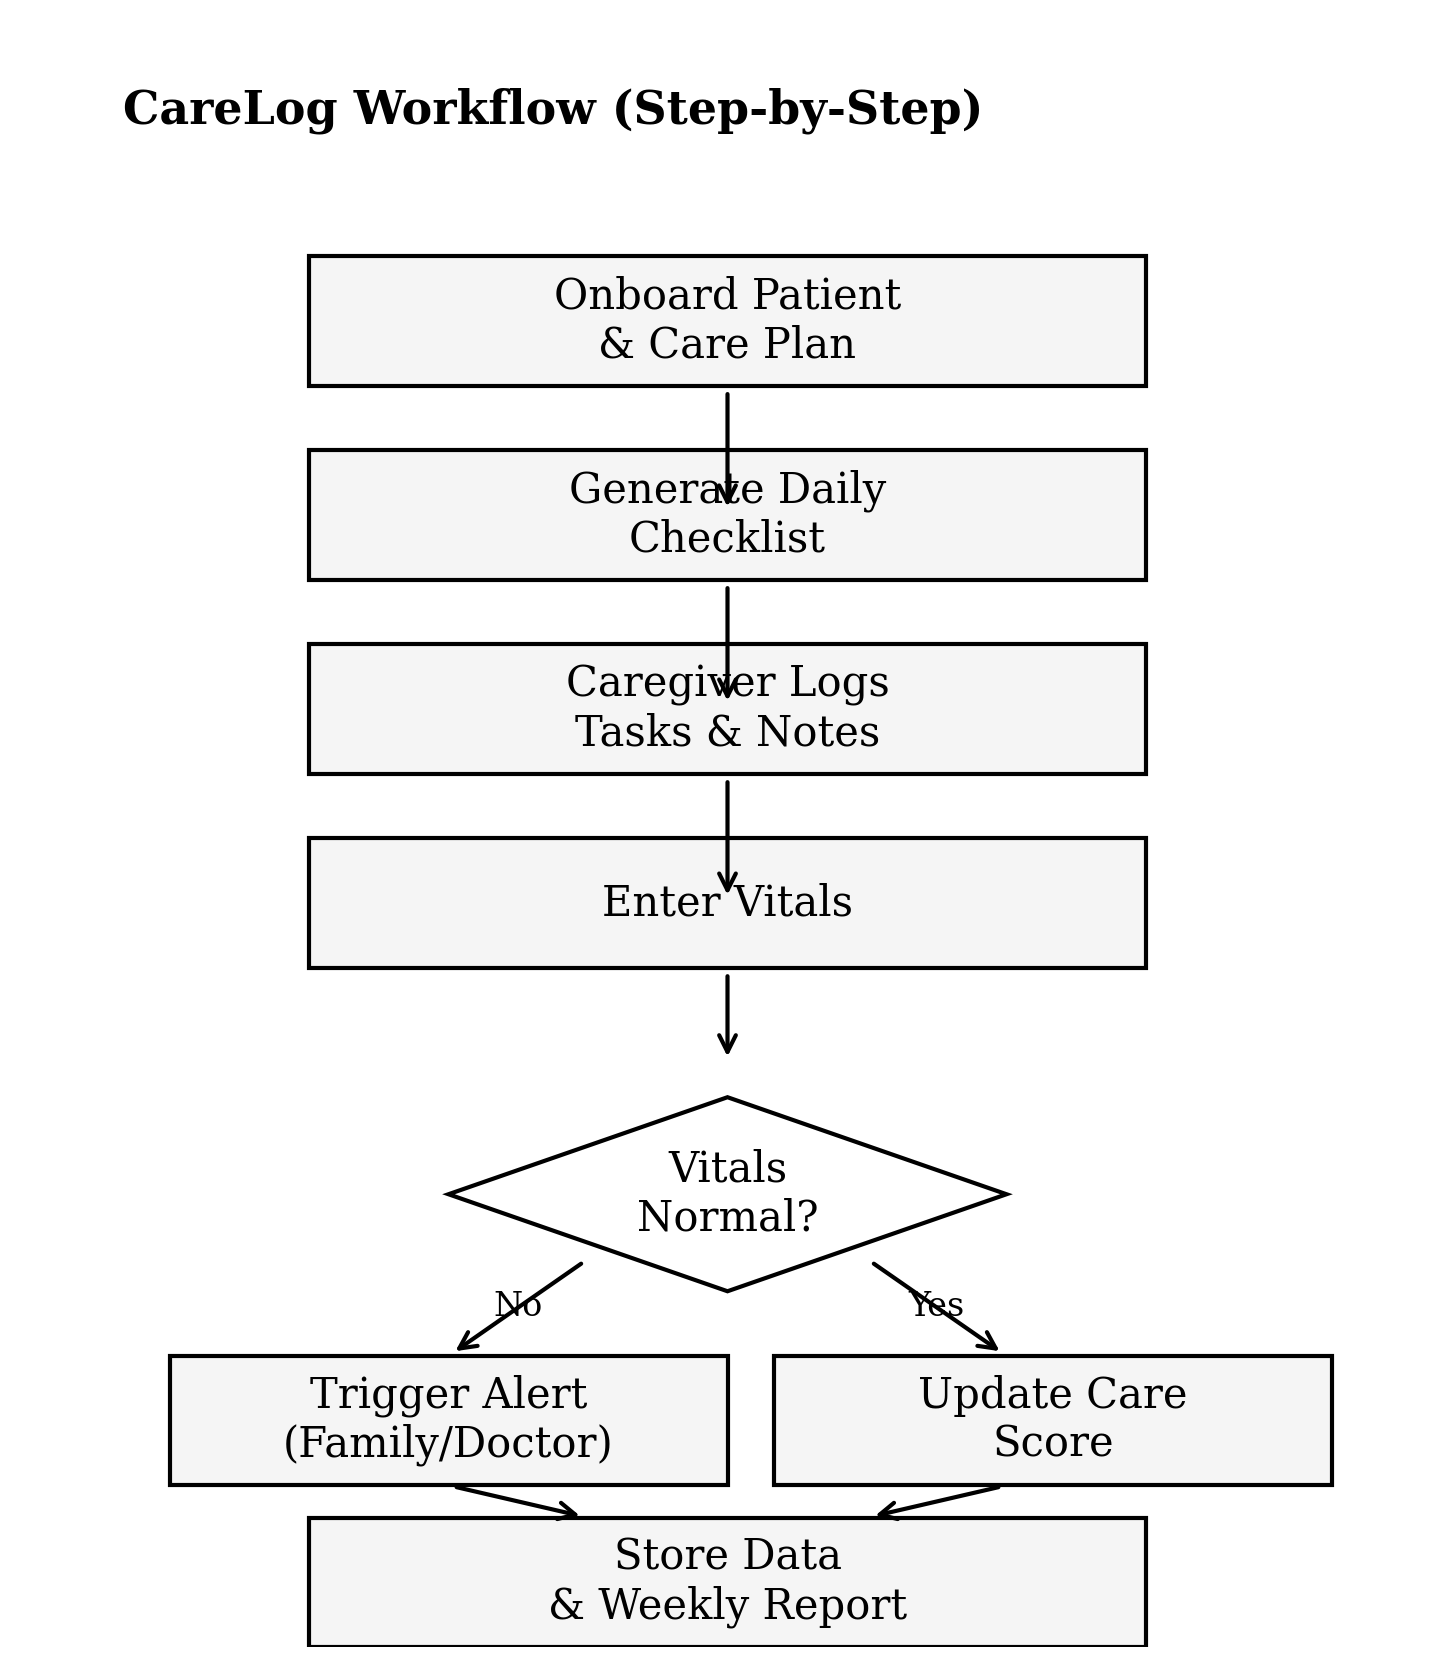
\includegraphics[width=\columnwidth]{output/figures/fig3_carelog_workflow.png}}
\caption{CareLog Workflow (Step by Step).}
\label{fig:workflow}
\end{figure}

\subsection{Data Model}
Core entities include patient profiles, care plans, daily tasks, vitals records, observations, alerts, and weekly reports. Each record includes timestamps and the role that created it. This structure supports traceability and reporting.

\subsection{Vitals Validation and Alerts}
Vitals are checked against safe thresholds. If a value crosses the safe range, the system generates an alert for the family and doctor. Alerts include the vital value, time, and source to support quick review.

\subsection{Care Score and Weekly Report}
A daily care score is computed based on task completion and vitals status. At the end of the week, the system compiles tasks, vitals, alerts, and observations into a single report for review.

\begin{table}[htbp]
\caption{CareLog Modules and Purpose}
\begin{center}
\begin{tabular}{|p{3.5cm}|p{4.2cm}|}
\hline
\textbf{Module} & \textbf{Purpose} \\
\hline
User Authentication & Role based access control \\
Patient Onboarding & Create care plan and schedule \\
Task and Reminder & Daily checklist and reminders \\
Vitals Monitoring & Record and validate vitals \\
Alert and Notification & Real time abnormal alerts \\
Care Score & Daily summary indicator \\
Weekly Report & Generate weekly care report \\
Doctor and Family Dashboard & Review logs and alerts \\
\hline
\end{tabular}
\label{tab:modules}
\end{center}
\end{table}

\section{Results and Discussion}
The CareLog prototype supports daily task logging, vitals entry, observations, and shift handoff notes. Alerts are generated when abnormal vitals are recorded, and the alerts appear immediately for families and doctors. Weekly reports summarize tasks, vitals trends, and alerts in a compact format. The checklist flow reduces typing and makes logging fast. Voice input helps caregivers record longer handoff notes without extra effort. The system improves continuity by replacing verbal handoffs with structured logs and improves visibility by providing daily dashboards and weekly summaries.

The caregiver dashboard includes the care plan, daily checklist, and progress view, as shown in Fig.~\ref{fig:dashboard}.

\begin{figure}[htbp]
\centering
\fbox{\parbox[c][4cm][c]{\columnwidth}{\centering Dashboard with care plan screenshot (placeholder)}}
\caption{Caregiver dashboard with care plan and daily checklist.}
\label{fig:dashboard}
\end{figure}

The alert system highlights abnormal vitals and missed tasks, as shown in Fig.~\ref{fig:alerts}.

\begin{figure}[htbp]
\centering
\fbox{\parbox[c][4cm][c]{\columnwidth}{\centering Alert system screenshot (placeholder)}}
\caption{Alert system view for abnormal vitals.}
\label{fig:alerts}
\end{figure}

The weekly report summarizes care activities and vitals trends, as shown in Fig.~\ref{fig:weekly}.

\begin{figure}[htbp]
\centering
\fbox{\parbox[c][4cm][c]{\columnwidth}{\centering Weekly PDF report screenshot (placeholder)}}
\caption{Weekly PDF report summary.}
\label{fig:weekly}
\end{figure}

\begin{table}[htbp]
\caption{Expected Results Compared to Existing Systems}
\begin{center}
\begin{tabular}{|p{2.6cm}|p{2.6cm}|p{2.6cm}|}
\hline
\textbf{Feature} & \textbf{Existing Systems} & \textbf{CareLog} \\
\hline
Caretaker coordination & Manual or verbal & Structured and digital \\
Real time monitoring & Limited & Alerts on abnormal vitals \\
Doctor visibility & Occasional & Weekly report and alerts \\
Data tracking & Unstructured & Organized and stored \\
Weekly reports & Rare & Automatic weekly summary \\
Hardware dependency & Often required & Not required \\
\hline
\end{tabular}
\label{tab:results}
\end{center}
\end{table}

\section{Conclusion}
CareLog is a multi role care coordination platform for home based elderly monitoring. It replaces unstructured handoffs with structured daily logs, validates vitals with real time alerts, and provides weekly summaries for clinical review. The system improves visibility for family members and doctors without relying on hardware devices.

\section{Future Scope}
Future work will include caregiver field trials, stronger offline support, multilingual voice input, and optional integration with wearable devices. Another direction is interoperability with clinical systems through standard health data formats.

\section*{Acknowledgment}
We thank Mrs. Ch. Sreedevi for her guidance and feedback.

\begin{thebibliography}{00}
\bibitem{b1} M. Kelley et al., ``Mobile health apps, family caregivers, and care planning: Scoping review,'' Journal of Medical Internet Research, 2024.
\bibitem{b2} T. Shi et al., ``Large language models in critical care medicine: Scoping review,'' JMIR Medical Informatics, 2025.
\bibitem{b3} R. Gayathri et al., ``Comprehensive health assessment using ensemble deep learning for remote patient monitoring with IoT,'' Scientific Reports, 2024.
\bibitem{b4} N. Dao et al., ``Generative AI for automated data extraction from unstructured medical text,'' JAMIA Open, 2025.
\bibitem{b5} N. Turnbull et al., ``A mobile application for enhancing caregiver support and resource management,'' Healthcare, 2024.
\bibitem{b6} M. Alshammari et al., ``Advancing remote monitoring for patients with Alzheimer disease,'' JMIR Aging, 2025.
\bibitem{b7} V. K. Damera et al., ``Enhancing remote patient monitoring with AI driven IoMT and cloud computing technologies,'' Scientific Reports, 2025.
\bibitem{b8} V. Ntinopoulos et al., ``Large language models for data extraction from electronic health records,'' BMJ Health Care Informatics, 2024.
\bibitem{b9} J. Huang et al., ``A critical assessment of using ChatGPT for extracting structured data from clinical notes,'' npj Digital Medicine, 2024.
\bibitem{b10} F. Tsvetanov et al., ``Integrating AI technologies into remote monitoring patient systems,'' Engineering Proceedings, 2024.
\end{thebibliography}

\end{document}
